\appendix

\chapter{Rotating spin Hamiltonian}\label{app:rotating_spin_hamiltonian}

\chapter{Derivation of the CD coefficients for an arbitrary Ising graph}\label{app:arbitrary_ising_derivation}

An Ising Hamiltonian for $N$ spins and with both a transverse and longitudinal field can be written as:
\begin{equation}\label{eq:ising_hamiltonian}
    H(\lambda) = \sum_{i = 1}^{N-1}\sum_{j = i+1}^{N} J_{ij}(\lambda) \sz_i \sz_j + \sum_{i = 1}^{N} \Big( X_i(\lambda) \sx_i + Z_i(\lambda) \sz_i \Big)
\end{equation}
where the coefficients $J_{ij}$ correspond to couplings between spins $i$ and $j$. Systems like this can be viewed as undirected graphs, with each spin corresponding to a vertex and each coupling $J_{ij}$ denoting an edge between the corresponding spins. In the case of a weighted graph, the magnitude of each $J_{ij}$ can be viewed as the weight of the correspoding edge. This type of Hamiltonian, for specific values of $J_{ij}$, $X_i$ and $Z_i$ can be used to describe the two-spin annealing example of Sec.~\ref{sec:5.1_2spin_annealing}, the Ising chain from Sec.~\ref{sec:5.2_Ising_chain} and the frustrated spin model of Sec.~\ref{sec:}. 

The first order \acrref{LCD} ansatz is just single-spin operators:
\begin{equation}\label{eq:spin_agp_1storder}
    \AGP{\lambda}^{(1)} = \sum_{i = 1}^N \alpha_i(\lambda) \sy_i
\end{equation}
and the second order can be split up into 4 separate symmetries of operators:
\begin{equation}\label{eq:spin_agp_2ndorder}
        \AGP{\lambda}^{(2)} = \sum_{i = 1}^{N-1}\sum_{j = i+1}^{N} \Big( \gamma_{ij}(\lambda) \sx_i \sy_j + \Bar{\gamma}_{ij}(\lambda) \sy_i \sx_j + \zeta_{ij}(\lambda) \sz_i \sy_j + \Bar{\zeta}_{ij}(\lambda) \sy_i \sz_j \Big).
\end{equation}

What follows is a derivation that one might call `messy' on a good day. The first order commutators are computed as follows:
\begin{equation}\label{eq:first_order_AGP_commutator}
        i\comm{\alpha_i \sy_i}{H} = 2\alpha_i \Big[ \sum_{j = i+1}^{N} - J_{ij} \Big( \sx_i \sz_j + \sz_i \sx_j \Big) + X_i \sz_i - Z_i \sx_i \Big],
\end{equation}
where I have omitted the dependence on $\lambda$ of the terms. The second order expansions, sadly, look like this:
\begin{equation}
    \begin{aligned}
        i\comm{\gamma_{ij} \sx_i \sy_j}{H(\lambda)} &= 2\gamma_{ij} \Big[ \sum_{k = 1}^{i-1} (J_{ki} \sz_k \sy_i \sy_j - J_{kj} \sz_k \sx_i \sx_j)  + \sum_{k = i + 1}^{j-1} (J_{ik} \sy_i \sz_k \sy_j - J_{kj} \sx_i \sz_k \sx_j) \\ 
        &+ \sum_{k = j + 1}^N (J_{ik} \sy_i \sy_j \sz_k - J_{jk} \sx_i \sx_j \sz_k) + Z_i \sy_i \sy_j + X_j \sx_i \sz_j - Z_j \sx_i \sx_j \Big] \\
        i\comm{\Bar{\gamma}_{ij} \sy_i \sx_j}{H} &= 2\Bar{\gamma}_{ij} \Big[ \sum_{k = 1}^{i-1} (J_{kj} \sz_k \sy_i \sy_j - J_{ki} \sz_k \sx_i \sx_j) + \sum_{k = i + 1}^{j-1} (J_{kj} \sy_i \sz_k \sy_j - J_{ik} \sx_i \sz_k \sx_j) \\ 
        &+ \sum_{k = j + 1}^N (J_{jk} \sy_i \sy_j \sz_k - J_{ik} \sx_i \sx_j \sz_k)+ Z_j \sy_i \sy_j + X_i \sz_i \sx_j - Z_i \sx_i \sx_j \Big] \\ 
        i\comm{\zeta_{ij} \sz_i \sy_j}{H(\lambda)} &= 2\zeta_{ij} \Big[ -\sum_{k = 1}^{i-1} J_{kj} \sz_k \sz_i \sx_j - \sum_{k = i + 1}^{j-1} J_{kj} \sz_i \sz_k \sx_j - \sum_{k = j + 1}^N J_{jk} \sz_i \sx_j \sz_k  \\
        &- J_{ij} \sx_j - X_i \sy_i \sy_j + X_j \sz_i \sz_j - Z_j \sz_i\sx_j \Big] \\
        i\comm{\Bar{\zeta}_{ij} \sy_i \sz_j}{H(\lambda)} &= 2\Bar{\zeta}_{ij} \Big[ - \sum_{k = 1}^{i-1} J_{ki} \sz_k \sx_i \sz_j - \sum_{k = i + 1}^{j-1} J_{ik} \sx_i \sz_k \sz_j 
        - \sum_{k = j + 1}^N J_{ik} \sx_i \sz_j \sz_k \\
        &- J_{ij} \sx_i - X_j \sy_i \sy_j + X_i \sz_i \sz_j - Z_i \sx_i \sz_j \Big]
    \end{aligned}
\end{equation}
Combined, the above commutators along with the coefficients of $\dlambda H$ give the operator $G_{\lambda}(\AGP{\lambda}^{(1,2)})$ for an ansatz \acrref{AGP} constructed from both single- and two-spin operators (as per Eq.~\eqref{eq:G_operator}):
\begin{equation}\label{eq:ising_graph_G_operator}
    \begin{aligned}
        G_{\lambda}(\AGP{\lambda}^{(1,2)}) &= \sum_{i=1}^N \Bigg[ (\dot{X}_i - 2\alpha_i Z_i - 2\sum_{j=1}^{i-1} J_{ji}\zeta_{ji} - 2\sum_{j=i+1}^N J_{ij}\zetabar_{ij})\sx_i \\
        &+ (\dot{Z}_i + 2\alpha_i X_i)\sz_i \Bigg] \\
        &+ \sum_{i = 1}^{N-1} \sum_{j = i+1}^{N} \Bigg[(\dot{J}_{ij} + 2\zeta_{ij} X_j + 2\zetabar_{ij} X_i)\sz_i\sz_j \\
        &+ (2\gamma_{ij}Z_i + 2\gammabar_{ij} Z_j - 2 \zeta_{ij} X_i - 2 \zetabar_{ij} X_j)\sy_i\sy_j \\
        &+ (2\gamma_{ij}Z_j + 2\gammabar_{ij} Z_i)\sx_i\sx_j \\
        &+ (-2\alpha_i J_{ij} + 2\gamma_{ij}X_j - 2\zetabar_{ij} Z_i)\sx_i\sz_j \\
        &+ (-2\alpha_j J_{ij} + 2\gammabar_{ij}X_i - 2\zeta_{ij} Z_j)\sz_i\sx_j \\
        &+ \sum_{k = 1}^{i-1} \Big[ (2\gamma_{ij}J_{ki} + 2\gammabar_{ij} J_{kj})\sz_k\sy_i\sy_j + (2\gamma_{ij}J_{kj} + 2\gammabar_{ij} J_{ki})\sz_k\sx_i\sx_j \\
        &+ (- 2 \zeta_{ij} J_{kj} - 2 \zeta_{kj}J_{ij})\sz_k\sz_i\sx_j \Big] \\
        &+ \sum_{k = i+1}^{j-1} \Big[ (2\gamma_{ij}J_{ik} + 2\gammabar_{ij} J_{kj})\sy_i\sz_k\sy_j + (2\gamma_{ij}J_{kj} \\
        &+ 2\gammabar_{ij} J_{ik})\sx_i\sz_k\sx_j + (- 2 \zetabar_{ij} J_{ik} - 2 \zeta_{ik}J_{ij})\sz_k\sx_i\sz_j \Big] \\
        &+ \sum_{k = j+1}^N \Big[ (2\gamma_{ij}J_{ik} + 2\gammabar_{ij} J_{jk})\sy_i\sy_j\sz_k + (2\gamma_{ij}J_{jk} + 2\gammabar_{ij} J_{ik})\sx_i\sx_j\sz_k \\
        &+ (- 2 \zetabar_{ij} J_{ik} - 2 \zetabar_{ik}J_{ij})\sz_i\sx_j\sz_k \Big] \Bigg].
    \end{aligned}
\end{equation}
In order to find the coupled set of equations that allow us to compute each of the coefficients in the approximate \acrref{AGP} according to the \acrref{LCD} approach, we need to minimise the action $\mathcal{S} = \Tr[G_{\lambda}^2]$ with respect to each of the coefficients. As the Pauli operators and their tensor products are traceless, this means that the action is merely the sum of the squares of all the orthogonal operator coefficients of $G_{\lambda}$. Minimising $\mathcal{S}$ with respect to each $\alpha_i$ gives:
\begin{equation}\label{eq:ising_graph_minimise_alpha}
    \begin{aligned}
        &\alpha_i \Big[2Z_i^2 + 2X_i^2 + \sum_{j = 1}^{i-1}2J_{ji}^2 + \sum_{i+1}^{N}2J_{ij}^2 \Big] \\
        \sum_{j = i+1}^N &\gamma_{ij} \Big[ -2J_{ij}X_j \Big] + \sum_{j = 1}^{i-1} \gammabar_{ji} \Big[ -2J_{ji}X_j \Big] \\
        \sum_{j = i+1}^N &\zetabar_{ij} \Big[ 4J_{ij}Z_i \Big] + \sum_{j = 1}^{i-1} \zeta_{ji} \Big[4 J_{ji}Z_i \Big] \\
        &= Z_i \dot{X}_i - X_i \dot{Z}_i,
    \end{aligned}
\end{equation}
where $i$ is fixed. Fixing $i$ and $j$ and minimising with respect to each $\gamma_{ij}$ gives:
\begin{equation}\label{eq:ising_graph_minimise_gamma}
    \begin{aligned}
        &\alpha_i\Big[ -X_j J_{ij} \Big] + \zeta_{ij}\Big[ -  X_i Z_i\Big] + \zetabar_{ij} \Big[ -2 X_j Z_i \Big] \\
        + \: &\gamma_{ij} \Big[ Z_i^2 + Z_j^2 + X_j^2 + \sum_{k = 1}^{i-1} (J_{ki}^2 + J_{kj}^2) + \sum_{k = i+1}^{j-1} (J_{ik}^2 + J_{kj}^2) + \sum_{k = j+1}^N (J_{ik}^2 + J_{jk}^2) \Big] \\
        + \: &\gammabar_{ij} \Big[ 2 Z_i Z_j + \sum_{k = 1}^{i-1} 2J_{ki}J_{kj} + \sum_{k = i+1}^{j-1} 2J_{ik}J_{kj} + \sum_{k = j+1}^N 2J_{ik}J_{jk} \Big] = 0
    \end{aligned}
\end{equation}
and likewise for each $\gammabar$:
\begin{equation}\label{eq:ising_graph_minimise_gammabar}
    \begin{aligned}
        &\alpha_j\Big[ -X_i J_{ij} \Big] + \zeta_{ij}\Big[ - 2 X_i Z_j\Big] + \zetabar_{ij} \Big[ - X_j Z_j \Big] \\
        + \: &\gammabar_{ij} \Big[ Z_i^2 + Z_j^2 + X_i^2 + \sum_{k = 1}^{i-1} (J_{ki}^2 + J_{kj}^2) + \sum_{k = i+1}^{j-1} (J_{ik}^2 + J_{kj}^2) + \sum_{k = j+1}^N (J_{ik}^2 + J_{jk}^2) \Big] \\
        + \: &\gamma_{ij} \Big[ 2 Z_i Z_j + \sum_{k = 1}^{i-1} 2J_{ki}J_{kj} + \sum_{k = i+1}^{j-1} 2J_{ik}J_{kj} + \sum_{k = j+1}^N 2J_{ik}J_{jk} \Big] = 0.
    \end{aligned}
\end{equation}
Finally, for fixed $i$, $j$, we minimise with respect to $\zeta_{ij}$:
\begin{equation}\label{eq:ising_graph_minimise_zeta}
    \begin{aligned}
        &\alpha_j\Big[ 4 Z_j J_{ij} \Big] + \gamma_{ij}\Big[ - 2 X_i Z_i\Big] + \gammabar_{ij} \Big[ - 4 X_i Z_j \Big] \\
        + \: &\zeta_{ij} \Big[ 2 Z_j^2 + 2X_i^2 + 2X_j^2 + \sum_{k = 1}^{i-1} 2 J_{kj}^2 + \sum_{k = i+1}^{j-1} 2 J_{jk}^2 \Big] + \zetabar_{ij}\Big[ 4 X_i X_j \Big] \\
        + \sum_{k = 1}^{i-1} &\zeta_{kj}\Big[ 2 J_{ij} J_{kj} \Big] + \sum_{k = 1}^{j-1} \zeta_kj \Big[2 J_{ij}J_{kj}\Big] \\
        + \sum_{k = i +1}^{j-1} &\zetabar_{jk} 2 J_{ij} J_{jk} + \sum_{k = j +1}^N \zetabar_{jk} 2 J_{ij} J_{jk} = J_{ij} \dot{X}_j - \dot{J}_{ij} X_j
    \end{aligned}
\end{equation}
and with respect to $\zetabar_{ij}$:
\begin{equation}\label{eq:ising_graph_minimise_zetabar}
    \begin{aligned}
        &\alpha_i\Big[ 4 Z_i J_{ij} \Big] + \gamma_{ij}\Big[ - 4 X_j Z_i\Big] + \gammabar_{ij} \Big[ - 2 X_j Z_j \Big] \\
        + \: &\zetabar_{ij} \Big[ 2 Z_i^2 + 2X_i^2 + 2X_j^2 + \sum_{k = i+1}^{j-1} 2 J_{ik}^2 + \sum_{k = j+1}^N 2 J_{ik}^2 \Big] + \zeta_{ij}\Big[ 4 X_i X_j \Big] \\
        + \sum_{k = i+1}^N &\zetabar_{ik}\Big[ 2 J_{ij} J_{ik} \Big] + \sum_{k = j+1}^N \zetabar_ik \Big[2 J_{ij}J_{ik}\Big] \\
        + \sum_{k = 1}^{i-1} &\zeta_{ki} 2 J_{ij} J_{ki} + \sum_{k = i+1}^{j-1} \zeta_{ik} 2 J_{ij} J_{ik} = J_{ij} \dot{X}_i - \dot{J}_{ij} X_i.
    \end{aligned}
\end{equation}

Armed with this knowledge, we can now explore the non-adiabatic effects generated by one- and two-spin operators on any random time-dependent Ising graph Hamiltonian. 

\chapter{More details and plots for the higher order AGP chapter}\label{app:higher_order_AGP}

I have so much stuff to add here, might just leave some here for now. 

\begin{figure}[t]
\centering
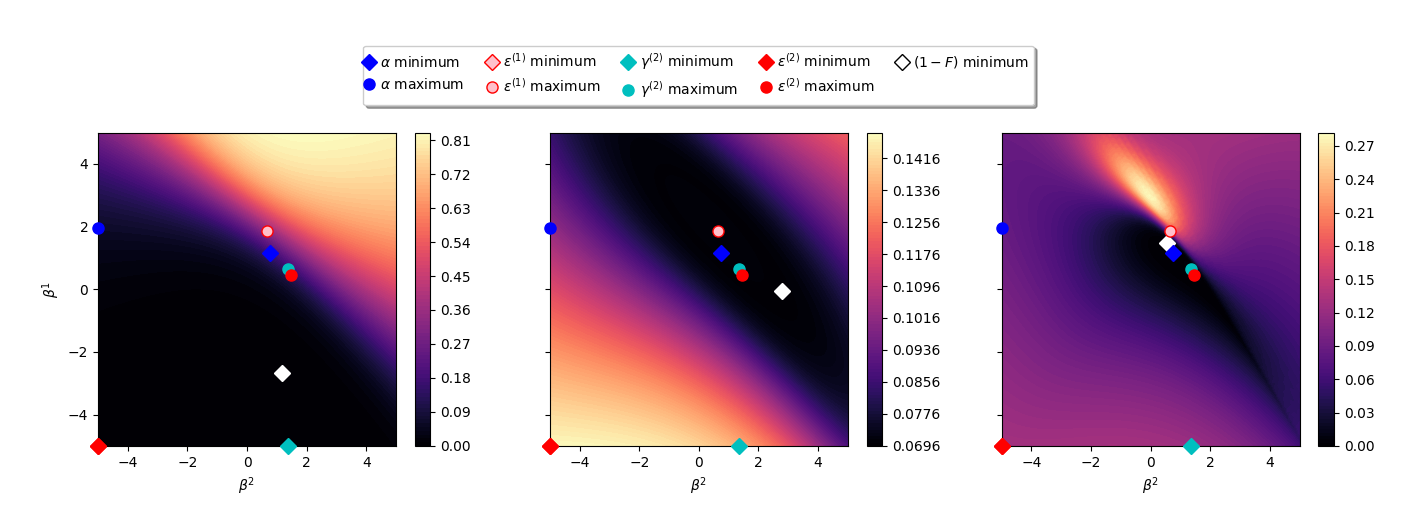
\includegraphics[width=\linewidth]{images/2_spins_Integrals_no_norm_final.png} \caption{Placeholder: integral unscaled}\label{fig:}
\end{figure}

\begin{figure}[t]
\centering
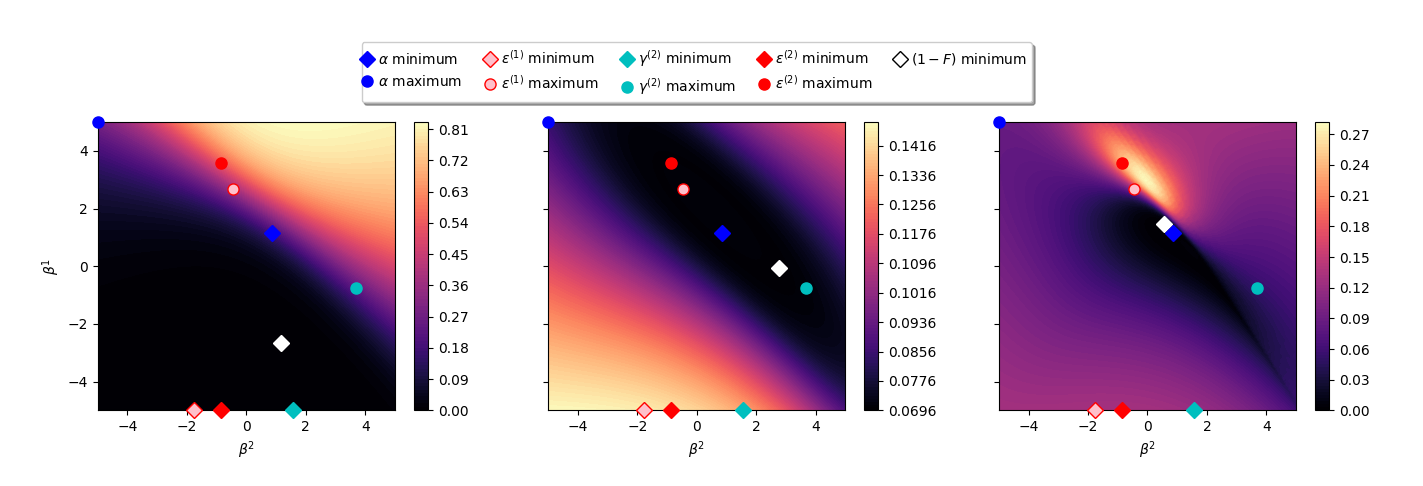
\includegraphics[width=\linewidth]{images/2spin_Maximums_no_norm_final} \caption{Placeholder: max amplitude unscaled}\label{fig:}
\end{figure}

\begin{figure}[t]
\centering
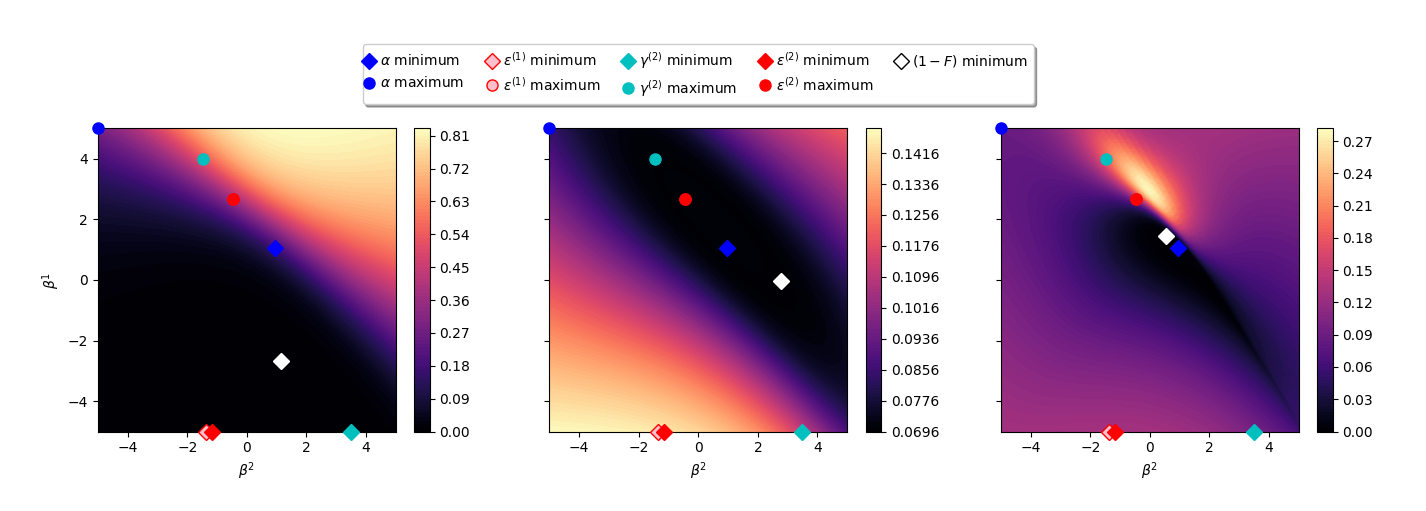
\includegraphics[width=\linewidth]{images/2spins_Maximums_scaled_by_norm_final.png} \caption{Placeholder: max amplitude scaled by Hamiltonian norm}\label{fig:}
\end{figure}

